\documentclass[a4paper]{article}
\usepackage[utf8]{inputenc}
\usepackage{alphabeta}
\usepackage{graphicx}
\usepackage[section]{placeins}
\usepackage{float}
\usepackage{amsmath}
\usepackage{listings}
\usepackage{xcolor}
\usepackage{amsmath}
\usepackage{extarrows}
\usepackage{amssymb}
\usepackage{verbatim}
\usepackage{enumerate}
\usepackage{eurosym}
\usepackage{svg}
\usepackage{varwidth}
\usepackage{moreverb}

\definecolor{codegreen}{rgb}{0,0.6,0}
\definecolor{codegray}{rgb}{0.5,0.5,0.5}
\definecolor{codepurple}{rgb}{0.58,0,0.82}
\definecolor{backcolour}{rgb}{0.95,0.95,0.92}

\def\verbatimtabsize{4}

\lstdefinestyle{mystyle}{
    backgroundcolor=\color{backcolour},   
    commentstyle=\color{codegreen},
    keywordstyle=\color{magenta},
    numberstyle=\tiny\color{codegray},
    stringstyle=\color{codepurple},
    basicstyle=\ttfamily\footnotesize,
    breakatwhitespace=false,         
    breaklines=true,                 
    captionpos=b,                    
    keepspaces=true,                 
    numbers=left,                    
    numbersep=5pt,                  
    showspaces=false,                
    showstringspaces=false,
    showtabs=false,                  
    tabsize=2
}

\lstset{style=mystyle}

\setlength{\parindent}{0pt}
\setlength{\parskip}{1em}
\setlength{\jot}{4mm}

\title{Συστήματα Μικροϋπολογιστών \\ 3η σειρά ασκήσεων}
\author{Νικόλαος Παγώνας, el18175 \\ Αναστάσιος Παπαζαφειρόπουλος, el18079}
\date{}

\begin{document}

\maketitle

\subsection*{1η άσκηση}
Η 1η άσκηση, μαζί με τα κατάλληλα σχόλια, βρίσκεται στο αρχείο \texttt{ex1.8085}.
Για λόγους πληρότητας παρατίθεται και εδώ.

\verbatimtabinput{ex1.8085}

\subsection*{2η άσκηση}
Η 2η άσκηση, μαζί με τα κατάλληλα σχόλια, βρίσκεται στο αρχείο \texttt{ex2.8085}.
Για λόγους πληρότητας παρατίθεται και εδώ.

\verbatimtabinput{ex2.8085}
\subsection*{3η άσκηση}
Η 3η άσκηση, μαζί με τα κατάλληλα σχόλια, βρίσκεται στο αρχείο \texttt{ex3.8085}.
Για λόγους πληρότητας παρατίθεται και εδώ.

\verbatimtabinput{ex3.8085}

\subsection*{4η άσκηση}

Η διακοπή συμβαίνει στο μέσο της εντολής \texttt{CALL 0880H}, οπότε θα ολοκληρωθεί η εκτέλεση της τρέχουσας εντολής. Η τρέχουσα τιμή του \texttt{Program Counter} (\texttt{0800Η}) αποθηκεύεται στη στοίβα, ο δείκτης στοίβας ανεβαίνει δύο θέσεις πάνω και στον μετρητή προγράμματος καταχωρείται η διεύθυνση \texttt{0880Η}. Στη συνέχεια, σώζεται η τιμή του \texttt{Program Counter} και η κατάσταση του \texttt{8085}, ενώ εκτελείται η ρουτίνα εξυπηρέτησης της διακοπής \texttt{RST 7.5}. Δηλαδή, η τιμή του \texttt{PC} αποθηκεύεται ξανά στη στοίβα, ο \texttt{SP} ανεβαίνει άλλες δύο θέσεις πάνω και στον \texttt{PC} καταχωρείται η διεύθυνση της διακοπής για να εκτελεστεί η σχετική ρουτίνα.  Όταν ολοκληρωθεί η εκτέλεση της ρουτίνας εξυπηρέτησης της διακοπής, η διεύθυνση που βρίσκεται στην κορυφή της στοίβας (\texttt{0880Η}) επανέρχεται στον \texttt{PC}, ο \texttt{SP} κατεβαίνει δύο θέσεις κάτω και εκτελείται η ρουτίνα που αρχίζει από τη διεύθυνση \texttt{0880Η}, σύμφωνα με την εντολή \texttt{CALL 0880H}. Αφού ολοκληρωθεί η εκτέλεση και της τελευταίας ρουτίνας, η διεύθυνση στην κορυφή της στοίβας (\texttt{0800Η}) επαναφέρεται στον \texttt{PC}, ο \texttt{SP} κατεβαίνει 2 θέσεις κάτω και συνεχίζεται η εκτέλεση του προγράμματος από τη διεύθυνση \texttt{0801Η}. Η όλη διαδικασία αποτυπώνεται καλύτερα παρακάτω, όπου εμφανίζονται σχηματικά τα περιεχόμενα \texttt{PC} και στοίβας.

\begin{figure}[H]
	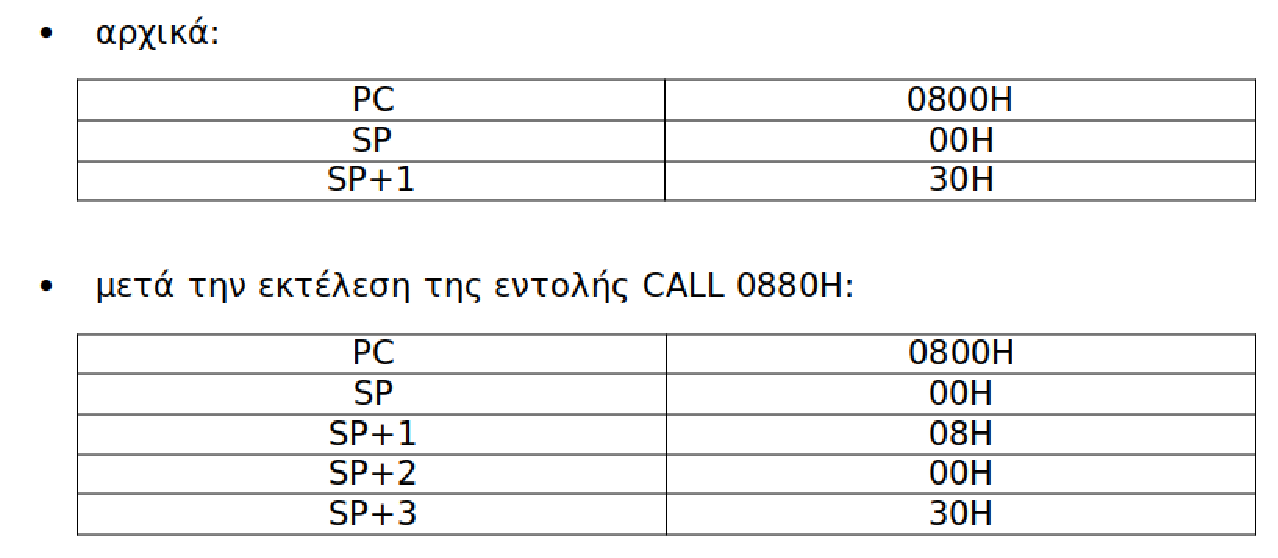
\includegraphics[width=\textwidth]{ex4a.pdf}
	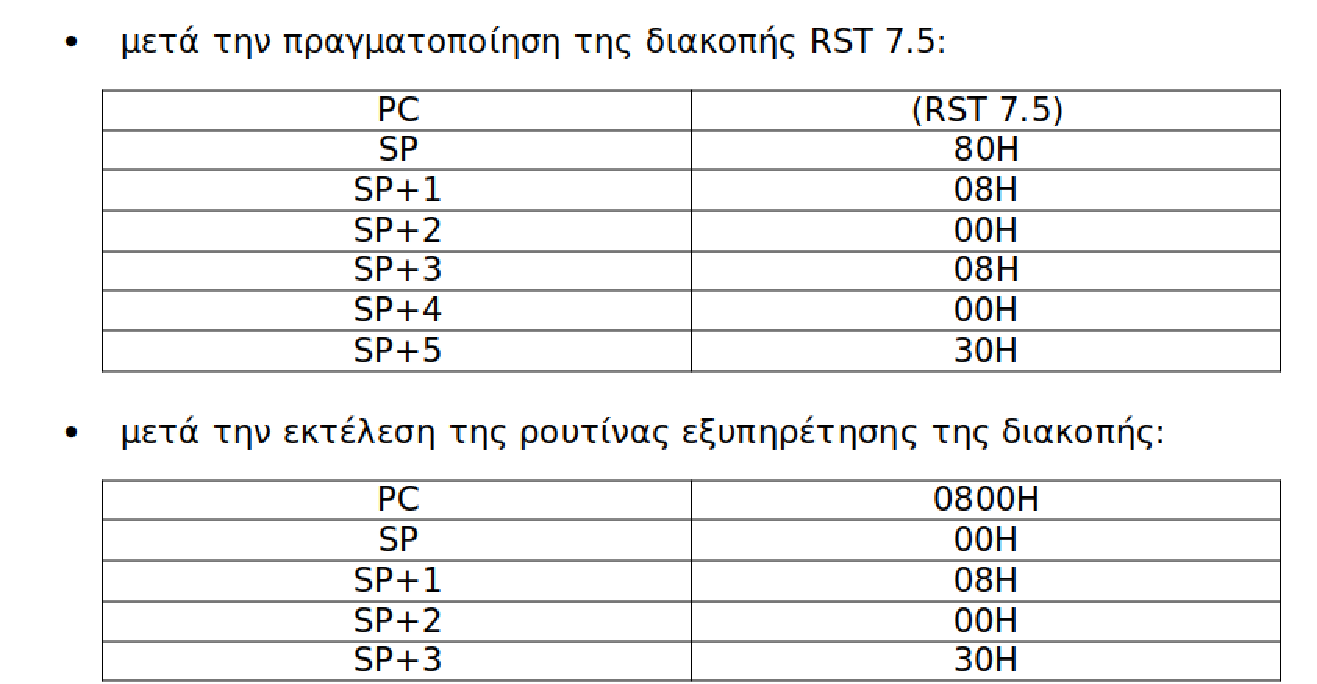
\includegraphics[width=\textwidth]{ex4b.pdf}
	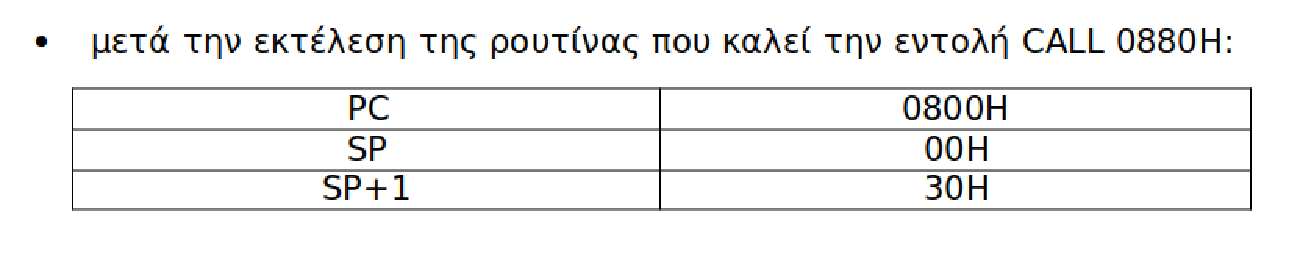
\includegraphics[width=\textwidth]{ex4c.pdf}	
\end{figure}

\subsection*{5η άσκηση}
Η 5η άσκηση, μαζί με τα κατάλληλα σχόλια, βρίσκεται στα αρχεία \texttt{ex5a.8085} και \texttt{ex5b.8085}, για υλοποίηση με και χωρίς διακοπές αντίστοιχα.
Για λόγους πληρότητας παρατίθεται και εδώ.

\textbf{Υλοποίηση με διακοπές}:
\verbatimtabinput{ex5a.8085}

\textbf{Υλοποίηση χωρίς διακοπές}:
\verbatimtabinput{ex5b.8085}


\end{document}
